\begin{figure}
	\begin{subfigure}{\linewidth}
	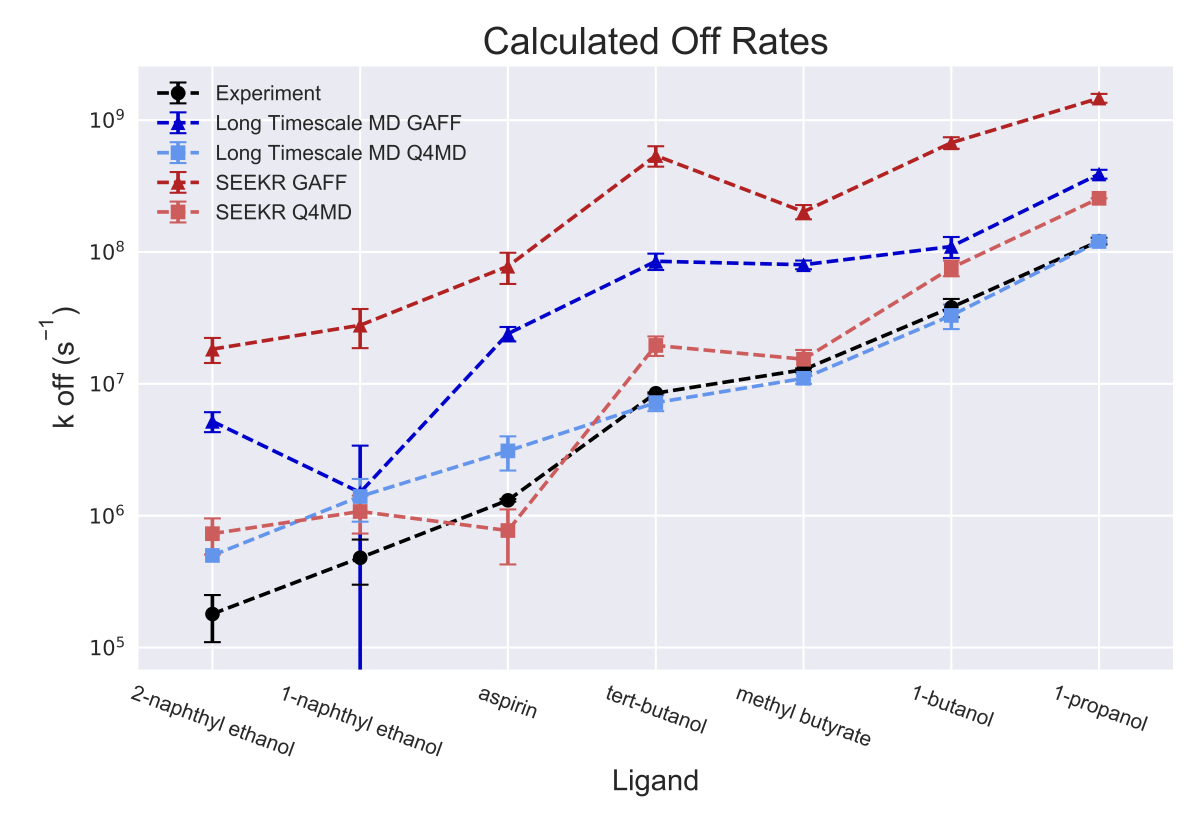
\includegraphics{images/off_scatter_resize.png}
	\caption{}
	\end{subfigure}

	\bigskip
	

	\begin{subfigure}{\linewidth}%<-- changed width
		%\centering
        %\renewcommand\tabularxcolumn[1]{m{#1}}% <-- added
        %\renewcommand\arraystretch{1.3}
        %\setlength\tabcolsep{2pt}% <-- added
    \begin{tabular}{
l  S[table-format = 2.3(3), separate-uncertainty] 
  S[table-format = 2.3(3), separate-uncertainty] 
 }%{\linewidth}%{*{4}{>{\centering\arraybackslash}X}}% <-- changed

\textbf{Method} & \textbf{Kendall} & \textbf{Spearman}  \\
\hline
      SEEKR GAFF      &    0.90(06)           &    0.96(04)            \\ 
      SEEKR Q4MD      &    0.81(09)           &    0.93(05)             \\ 
      Long Timescale MD GAFF      &    0.81(09)           &    0.93(04)                     \\ 
      Long Timescale MD Q4MD      &    01.00(05)           &    1.00(03)                     \\ 
     

    \end{tabular}
        \caption{}
	\end{subfigure}
	\caption{a) Experimental and calculated off rates for SEEKR GAFF and Q4MD forcefields as well as long timescale MD with both forcefields. b) Calculated rank correlation coefficients. Errors are determined with a bootstrapping analysis. }
	\label{fig: off_scatter}
\end{figure}